\begin{frame}{Privacy}
    \begin{block}{Motivation}
        One of the benefits of using blockchain technology is its transparency and accessibility. How do we protect users' private information? We followed the strategy proposed in the paper by encrypting the information in different portions.
    \end{block}
    
    \begin{block}{Technology}
        We used the \textbf{Asymmetric Encryption} strategy to encrypt each portion.
    \end{block}
    
    \vspace{5pt}
    
    \centering
    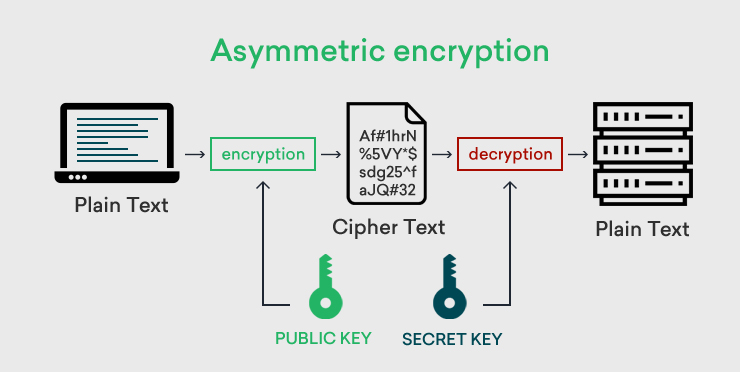
\includegraphics[width=0.65\linewidth]{images/encryption.jpg}
\end{frame}

\begin{frame}{Privacy}
    \begin{block}{Signatures}
        Data is encrypted both to guarantee user' \textbf{privacy} and to \textbf{avoid intrusions}.
        \begin{itemize}
            \item Knowing the seed of a MAM channel is enough for a malicious node to intrude
            \item Still, the asymmetric encryption allows to sign the \textbf{ciphertexts} with the private key
            \begin{itemize}
                \item [$\Rightarrow$] It is important to notice that \textbf{everybody} can \textbf{verify} a signature, as no key is needed
                \item [$\Rightarrow$] e.g., in our case the diagnostician is able to verify the correctness of the agents' transactions without the need of decrypting them
            \end{itemize}
        \end{itemize}
    \end{block}

    \begin{block}{Entities' Keys}
        Each entity has its own pair of private and public keys to have a one-to-one encryption.
        \begin{itemize}
            \item \textbf{Agents} use their keys to encrypt their personal information for the geosolver
            \item \textbf{Diagnosticians} use their keys to encrypt and sign the messages containing the positive agents' data, which can be decrypted by the geosolver only as well
            \item The \textbf{GeoSolver} uses its keys to decrypt both diagnosticians' and agents' messages
        \end{itemize}
        Additionally, as one-to-many encryption is not directly supported, the \textbf{GeoSolver} encrypts its data in order to be able to guarantee their authenticity, but these messages can be decrypted by anyone who possesses a shared private key.
    \end{block}
\end{frame}